\documentclass[aps,prb,reprint,showkeys,superscriptaddress]{revtex4-1}
\usepackage{subcaption}
\captionsetup{justification   = raggedright,
              singlelinecheck = false}
\usepackage{bm,graphicx,tabularx,array,booktabs,dcolumn,xcolor,microtype,multirow,amscd,amsmath,amssymb,amsfonts,physics,siunitx}
\usepackage[version=4]{mhchem}
\usepackage[utf8]{inputenc}
\usepackage[T1]{fontenc}
\usepackage{txfonts}
\usepackage[normalem]{ulem}
\usepackage{mleftright}

%%% Definition of colors for personal remark %%%
\newcommand{\todo}[1]{\textcolor{red}{#1}}
\newcommand{\ant}[1]{\textcolor{orange}{#1}}
\newcommand{\trashant}[1]{\textcolor{orange}{\sout{#1}}}

\usepackage[
	colorlinks=true,
    citecolor=blue,
    linkcolor=blue,
    filecolor=blue,      
    urlcolor=blue,	
    breaklinks=true
	]{hyperref}
\urlstyle{same}

%============================================================%
%%% NEWCOMMANDS %%%
%============================================================%

%============================================================%
%%% NEWCOMMANDS %%%
% ============================================================%

%%% This latex gather all the latex commands that I use to facilitate the writing of electronic structure manuscript, report...
%%% You can import these commands by adding the following line in you .text
%%% %============================================================%
%%% NEWCOMMANDS %%%
% ============================================================%

%%% This latex gather all the latex commands that I use to facilitate the writing of electronic structure manuscript, report...
%%% You can import these commands by adding the following line in you .text
%%% %============================================================%
%%% NEWCOMMANDS %%%
% ============================================================%

%%% This latex gather all the latex commands that I use to facilitate the writing of electronic structure manuscript, report...
%%% You can import these commands by adding the following line in you .text
%%% \input{commands}

%%% Latin %%%

\newcommand{\ie}{\textit{i.e.}~}
\newcommand{\eg}{\textit{e.g.}~}
\newcommand{\etal}{\textit{et al.}~}

%%% Operators %%%

\newcommand{\hH}{\Hat{H}} % Hamiltonian operator
\newcommand{\HN}{\Hat{\mathnormal{H}}_{\text{N}}} % Normal ordered Hamiltonian
\newcommand{\Hsim}{\hat{\bar{H}}} % Similarity transformed Hamiltonian
\newcommand{\hC}{\Hat{C}} % CI operator
\newcommand{\hT}{\Hat{T}} % Cluster operator
\newcommand{\T}[1]{\Hat{\mathnormal{T}}_{#1}} % Cluster operator of a given excitation number
\newcommand{\hsig}{\Hat{\sigma}} % Unitary cluster operator
\newcommand{\hK}{\Hat{K}} % Anti-hermitian orbital rotation operator
\newcommand{\hS}{\Hat{S}} % Anti-hermitian CI coefficients rotation operator
\newcommand{\hP}[1]{\Hat{\mathnormal{P}}_{#1}} % Permutation operators

\newcommand{\hE}{\Hat{E}} % Spin averaged single excitation operator
\newcommand{\cre}[1]{a_{#1}^\dagger} % Creation operator
\newcommand{\ani}[1]{a_{#1}} % Annihilation operator
\newcommand{\bcre}[1]{b_{#1}^\dagger} % Boson creation operator
\newcommand{\bani}[1]{b_{#1}} % Boson annihilation operator

\newcommand{\com}[2]{\mleft[#1,#2 \mright]} % Commutator

%%% Wave functions %%%



%%% Matrix and tensor elements %%%

\newcommand{\oa}{O_{\alpha}}
\newcommand{\ob}{O_{\beta}}
\newcommand{\eri}[2]{\braket{#1}{#2}} % Electron repulsion integral physician notation
\newcommand{\ceri}[2]{\mleft(#1|#2\mright)} % Electron repulsion integral chemist notation
\newcommand{\dbi}[2]{\mel{#1}{}{#2}} % Double bar integral
\newcommand{\kron}[1]{\delta_{#1}} % Kronecker delta

%%% Matrix %%%

\newcommand{\FC}[1]{F_{#1}^{\text{C}}} % Core Fock matrix
\newcommand{\FA}[1]{F_{#1}^{\text{A}}} % Active Fock matrix

%%% Text acronyms and abbreviations %%%

\newcommand{\FCI}{\text{FCI}}
\newcommand{\HF}{\text{HF}}
\newcommand{\MCSCF}{\text{MCSCF}}
\newcommand{\occ}{\text{occ}}
\newcommand{\vir}{\text{vir}}


\newcommand{\SupInf}{\textcolor{blue}{Supporting Information}}



%%% Latin %%%

\newcommand{\ie}{\textit{i.e.}~}
\newcommand{\eg}{\textit{e.g.}~}
\newcommand{\etal}{\textit{et al.}~}

%%% Operators %%%

\newcommand{\hH}{\Hat{H}} % Hamiltonian operator
\newcommand{\HN}{\Hat{\mathnormal{H}}_{\text{N}}} % Normal ordered Hamiltonian
\newcommand{\Hsim}{\hat{\bar{H}}} % Similarity transformed Hamiltonian
\newcommand{\hC}{\Hat{C}} % CI operator
\newcommand{\hT}{\Hat{T}} % Cluster operator
\newcommand{\T}[1]{\Hat{\mathnormal{T}}_{#1}} % Cluster operator of a given excitation number
\newcommand{\hsig}{\Hat{\sigma}} % Unitary cluster operator
\newcommand{\hK}{\Hat{K}} % Anti-hermitian orbital rotation operator
\newcommand{\hS}{\Hat{S}} % Anti-hermitian CI coefficients rotation operator
\newcommand{\hP}[1]{\Hat{\mathnormal{P}}_{#1}} % Permutation operators

\newcommand{\hE}{\Hat{E}} % Spin averaged single excitation operator
\newcommand{\cre}[1]{a_{#1}^\dagger} % Creation operator
\newcommand{\ani}[1]{a_{#1}} % Annihilation operator
\newcommand{\bcre}[1]{b_{#1}^\dagger} % Boson creation operator
\newcommand{\bani}[1]{b_{#1}} % Boson annihilation operator

\newcommand{\com}[2]{\mleft[#1,#2 \mright]} % Commutator

%%% Wave functions %%%



%%% Matrix and tensor elements %%%

\newcommand{\oa}{O_{\alpha}}
\newcommand{\ob}{O_{\beta}}
\newcommand{\eri}[2]{\braket{#1}{#2}} % Electron repulsion integral physician notation
\newcommand{\ceri}[2]{\mleft(#1|#2\mright)} % Electron repulsion integral chemist notation
\newcommand{\dbi}[2]{\mel{#1}{}{#2}} % Double bar integral
\newcommand{\kron}[1]{\delta_{#1}} % Kronecker delta

%%% Matrix %%%

\newcommand{\FC}[1]{F_{#1}^{\text{C}}} % Core Fock matrix
\newcommand{\FA}[1]{F_{#1}^{\text{A}}} % Active Fock matrix

%%% Text acronyms and abbreviations %%%

\newcommand{\FCI}{\text{FCI}}
\newcommand{\HF}{\text{HF}}
\newcommand{\MCSCF}{\text{MCSCF}}
\newcommand{\occ}{\text{occ}}
\newcommand{\vir}{\text{vir}}


\newcommand{\SupInf}{\textcolor{blue}{Supporting Information}}



%%% Latin %%%

\newcommand{\ie}{\textit{i.e.}~}
\newcommand{\eg}{\textit{e.g.}~}
\newcommand{\etal}{\textit{et al.}~}

%%% Operators %%%

\newcommand{\hH}{\Hat{H}} % Hamiltonian operator
\newcommand{\HN}{\Hat{\mathnormal{H}}_{\text{N}}} % Normal ordered Hamiltonian
\newcommand{\Hsim}{\hat{\bar{H}}} % Similarity transformed Hamiltonian
\newcommand{\hC}{\Hat{C}} % CI operator
\newcommand{\hT}{\Hat{T}} % Cluster operator
\newcommand{\T}[1]{\Hat{\mathnormal{T}}_{#1}} % Cluster operator of a given excitation number
\newcommand{\hsig}{\Hat{\sigma}} % Unitary cluster operator
\newcommand{\hK}{\Hat{K}} % Anti-hermitian orbital rotation operator
\newcommand{\hS}{\Hat{S}} % Anti-hermitian CI coefficients rotation operator
\newcommand{\hP}[1]{\Hat{\mathnormal{P}}_{#1}} % Permutation operators

\newcommand{\hE}{\Hat{E}} % Spin averaged single excitation operator
\newcommand{\cre}[1]{a_{#1}^\dagger} % Creation operator
\newcommand{\ani}[1]{a_{#1}} % Annihilation operator
\newcommand{\bcre}[1]{b_{#1}^\dagger} % Boson creation operator
\newcommand{\bani}[1]{b_{#1}} % Boson annihilation operator

\newcommand{\com}[2]{\mleft[#1,#2 \mright]} % Commutator

%%% Wave functions %%%



%%% Matrix and tensor elements %%%

\newcommand{\oa}{O_{\alpha}}
\newcommand{\ob}{O_{\beta}}
\newcommand{\eri}[2]{\braket{#1}{#2}} % Electron repulsion integral physician notation
\newcommand{\ceri}[2]{\mleft(#1|#2\mright)} % Electron repulsion integral chemist notation
\newcommand{\dbi}[2]{\mel{#1}{}{#2}} % Double bar integral
\newcommand{\kron}[1]{\delta_{#1}} % Kronecker delta

%%% Matrix %%%

\newcommand{\FC}[1]{F_{#1}^{\text{C}}} % Core Fock matrix
\newcommand{\FA}[1]{F_{#1}^{\text{A}}} % Active Fock matrix

%%% Text acronyms and abbreviations %%%

\newcommand{\FCI}{\text{FCI}}
\newcommand{\HF}{\text{HF}}
\newcommand{\MCSCF}{\text{MCSCF}}
\newcommand{\occ}{\text{occ}}
\newcommand{\vir}{\text{vir}}


\newcommand{\SupInf}{\textcolor{blue}{Supporting Information}}



\newcommand{\UOX}{Physical and Theoretical Chemical Laboratory, Department of Chemistry, University of Oxford, Oxford, OX1 3QZ, U.K.}

\begin{document}	

\title{An energy landscape perspective on CASSCF multiple solutions}

\author{Antoine \surname{Marie}}
\affiliation{\UOX}
\author{Hugh G.~A.~\surname{Burton}}
\affiliation{\UOX}

\begin{abstract}
\todo{Write an abstract.}
\end{abstract}

\keywords{\todo{Add keywords.}}

\maketitle

%=================================================================%
\section{Introduction}
\label{sec:intro}
% =================================================================%

State-specific (SS) electronic structure methods for excited states are on the rise. \cite{Gilbert_2008,Barca_2014,Thom_2008,Ye_2017,Barca_2018a,Thompson_2018,Hait_2020,Carter-Fenk_2020,Hait_2021,Mayhall_2010,Lee_2019,Kossoski_2021}
Their treatment of excited states on an equal footing to the ground state provides a natural way to compute relative energies such as excitation energies.
On the other hand, linear-response and equation-of-motion based methods are known to introduce a bias towards the ground state. \cite{McLachlan_1964,Runge_1984,Dreuw_2005,Burke_2005,Bartlett_2012,Helmich-Paris_2019}
However, this attractive property comes with a cost, namely one should be able to converge toward excited-state solutions of a given formalism.
While energy landscapes in electronic structure theory are mainly considered during minimization processes to target ground states, these higher-energy solutions has been shown to exist most often as non-zero index stationary points, \ie saddle points and maxima. \cite{Burton_2021}
While converging toward a minimum is somewhat straightforward, converging towards saddle points is much more subtle.
Moreover, in addition to these physical excited-state solutions, other spurious unphysical stationary points might exist on these landscapes.
Therefore, an accurate understanding of the underlying landscape of a given method helps to design algorithms targeting any stationary points, which we will refer to as state-specific algorithms. \cite{Burton_2022}

The Hartree-Fock (HF) \cite{Szabo_1996} energy landscape is now fairly well understood.\cite{Thompson_2018,Dong_2020,Burton_2021}
On this landscape one can find single-determinant approximations of excited states \cite{Gilbert_2008,Barca_2014} and quasi-diabatic states. \cite{Thom_2009}
In addition, when correlation is getting strong, additional symmetry-broken solutions may appear.\cite{Coulson_1949}
As a consequence the number of solution can vary with the geometry of the system.
One can find similar single-determinant approximations of excited states in the context of density functional theory (DFT). \cite{Hait_2020,Hait_2021}
Hait \etal have shown that minimizing the variance instead of the energy can provide an easier way of converging mean-field excited states, \cite{Hait_2020} see Ref.~\onlinecite{Burton_2022} for an extensive discussion on the advantages and flaws of variance-based minimization from an energy landscape perspective.
In addition, $\Delta$-DFT can access double excitations which are inherently out of range of time-dependent (TD) DFT \cite{Hait_2021} and provide a fairly good description of charge transfer excitations for which TDDFT is known to seriously fail. \cite{Tozer_2003,Dreuw_2004,Hait_2021} 

State-specific algorithms can also be developped for correlated methods such as coupled-cluster (CC). \cite{Shavitt_2009}
The CC energy landscape also exhibits higher-lying solutions corresponding to physical excited states. \cite{Jankowski_1994,Jankowski_1994a,Piecuch_2000,Mayhall_2010,Lee_2019,Kossoski_2021}
However, there are also stationary points associated with non-physical spurious solutions which need to be avoided in practice. \cite{Jankowski_1994,Jankowski_1994a,Piecuch_2000,Mayhall_2010,Kossoski_2021,Marie_2021a}
It is interesting to note that excited-state solutions exist in traditional CC theory although it is a projective method.
Moreover, it has been shown, by comparison with the variational CC landscape, that some of the unphysical CC solutions were due to this projective way of solving the equations. \cite{Marie_2021}
Here again, insights on the energy landscape have been useful to improve convergence toward CC excited states solutions, notably understanding the influence of the reference wave function on the basins of attraction. \cite{Jankowski_1995,Lee_2019,Marie_2021a}
$\Delta$-CC has been proved to give accurate energies for doubly excited states and double core excitations. \cite{Lee_2019}
It has also been shown that one can obtain excitation energies in agreement with equation-of-motion CCSDT (CC with single, double and triple excitations) using only $\Delta$-pCCD (CC restricted to closed-shell double excitations). \cite{Kossoski_2021}

The methods mentioned previously are known to fail dramatically in the presence of strong correlation. \cite{Jensen_2017}
The state-of-the-art method to treat static correlation in electronic structure is the multi-configuration self-consistent field (MCSCF) method in its complete active space (CAS) variant. \cite{Roos_2016}
The CASSCF method aims at optimizing the configuration interaction (CI) coefficients as well as the molecular orbitals of a trial wave function written as a linear combination of Slater determinants. \cite{Helgaker_2000,Roos_2016}
Therefore, the CASSCF ground state is a minimum with respect to these two sets of parameters and very powerful algorithm have been implemented to obtain this solution. \cite{Roos_1980,Werner_1985,Sun_2017,Kreplin_2019,Kreplin_2020}
Moreover, higher-lying stationary points corresponding to excited states have also been found on the CASSCF energy landscape (see the following paragraph).
However, so far converging consistently toward a given saddle point on this landscape is difficult to achieve in practice.
This is why the state-average (SA) approach is almost always used in practice to obtain approximate excited states within the CASSCF formalism.
In SA-CASSCF the energy of an average of $n$ states is minimized, hence an approximation for the $n$ lowest states of the system is obtained.
As a consequence these states are not true CASSCF stationary points because the orbitals are optimized for all states at the same time.

While being computationally simpler, the SA-CASSCF method is not without its own flaws. \cite{Zaitsevskii_1994,Helmich-Paris_2019} \todo{Find ref for this paragraph}
First, SA-CASSCF potential energy surfaces often show discontinuities if the average contains two states of different character therefore requiring different orbitals (for example the ground state and a charge-transfer excited state). \cite{Zaitsevskii_1994}
Secondly, SA-CASSCF can access excited states only within the CAS therefore it requires large active space to target high-lying states.
Moreover, because SA-CASSCF solutions are not true stationary points they cannot benefit from the Helmann-Feynman theorem.
These drawbacks of SA-CASSCF motivates the work towards a SS-CASSCF algorithm despite the difficulties associated with its developpement to overcome SA-CASSCF in difficult cases.

In their seminal work on the MCSCF stationary points, Olsen and co-workers used the Fletcher algorithm together with a second-order Newton-Raphson algorithm to target stationary points of a given index. \cite{Olsen_1982,Olsen_1983}
They observed that there are many of them and that convergence is very sensitive to the starting point.
In subsequent works, several criteria that a physically meaningful solution should fulfill have been introduced. \cite{Olsen_1983,Golab_1983,Golab_1985,Rizzo_1990}
Maybe the most troubling finding of these studies has been that sometimes for a given states two physical solutions, \ie matching all criteria, can be found. \cite{Rizzo_1990}
Multiple SS-CASSCF solutions have been found in further studies by other groups. \cite{Guihery_1997,Angeli_2003}
One observation shared by all these studies is that the basis set and the size of the CAS strongly influence the multiple solutions that they could find.
More recently, the group of Neuscamman tackled the problem of SS-CASSCF solution again. They developped an algorithm based on the generalized variational principle to target excited states on the CASSCF landscape. \cite{Tran_2019,Tran_2020,Hanscam_2021}
\todo{This paragraph needs improvements}

The aim of this work is to shed light on the SS-CASSCF landscape and its stationary points because we believe that a clear understanding of the multiple CASSCF solutions will facilitate future works on SS-CASSCF.
For example, confirming the presence (or absence) of unphysical solutions on this landscape, as well as understanding under what conditions these solutions exist, is of primary importance.
Moreover, it would be interesting to know whether SS-CASSCF can fix some flaws of the SA formalism, as the description of high-lying excited states out of the CAS or the description of avoided crossing, or not.
Finally, from a theoretical point of view, this study aims at further improving our understanding of electronic structure energy landscapes by understanding the mixing of the highly non-linear HF landscape with the linear degrees of freedom of the CI expansion.
In the next section, we will briefly review the CASSCF theory then we will present the computational details of this study in Sec.~\ref{sec:comp_details}.
Section~\ref{sec:excited} showcase the SS-CASSCF excited-state solutions in two simple examples, then we investigate the origin of unphysical solutions in Sec.~\ref{sec:spurious}.
Section~\ref{sec:static} shows how the solution space evolves in presence of static correlation.
Finally, we look at the behavior of SS-CASSCF solutions in the neighborhood of avoided crossings in Sec.~\ref{sec:avoided} before drawing conclusions in Sec~.\ref{sec:conclusion}.
Atomic units will be used throughout the manuscript.

%=================================================================%
\section{Theoretical background}
\label{sec:theoretical}
%=================================================================%

The exact solution $\ket{\Psi_{\FCI}}$, in a finite Hilbert space, of the non-relativistic electronic Schr\"odinger equation in the Born-Oppenheimer approximation
\begin{equation}
  \label{eq:schro_eq}
  \hH \ket{\Psi_{\FCI}} = E \ket{\Psi_{\FCI}},
\end{equation}
where $\hH$ is the electronic Hamiltonian, can be written as \cite{Szabo_1996}
\begin{equation}
  \label{eq:fci_wf}
  \ket{\Psi_{\FCI}} = \sum_I^{N_{det}} C_I\ket{I},
\end{equation}
\ie as a linear combination of $N_{det}$ Slater determinants $\ket{I}$.
The CI coefficients $C_I$ are determined by diagonalization of the Hamiltonian within the basis of Slater determinants.
An equivalent way to determine these coefficients is to find the stationary points of the energy
\begin{equation}
  \label{eq:fci_nrj}
  E = \frac{\mel{\Psi_{\FCI}}{\hH}{\Psi_{\FCI}}}{\braket{\Psi_{\FCI}}{\Psi_{\FCI}}},
\end{equation}
 with respect to their variation.
The number of CI coefficients $N_{det}$ to determine grows exponentially with the size of the underlying one-electron basis $K$ and the number of electrons $N$ and therefore can be determined only for small systems.

A natural way of approximating the exact wave function (\ref{eq:fci_wf}) is to truncate the sum to a number of determinants that we can handle. Then by diagonalization of the Hamiltonian within this finite subset of determinants we obtain an approximation of the exact solutions.
However, the resulting approximate wave functions will not be stationary points of the energy.
For a truncated CI expansion one needs to optimize the CI coefficients as for the complete expansion but also the coefficients $c_i^\mu$ of the molecular orbitals
\begin{equation}
  \label{eq:mo}
  \phi_i(\bm{x}) = \sum^K_\mu c_i^\mu \chi_{\mu}(\bm{x}),
\end{equation}
constituting the determinants. The $\chi_{\mu}(\bm{x})$ are the atomic orbitals which depend on the spin-spatial coordinate $\bm{x} = (\bm{r},\sigma)$ of an electron.
Optimizing the CI coefficients $C_I$ and the orbital coefficients $c_i^\mu$ for a given truncation of Eq.~(\ref{eq:fci_wf}) defines the MCSCF ans\"atz.
The CASSCF ans\"atz is a special case of the MCSCF one in which the truncation is done according to an active space defined by the user.
More precisely, the determinants included in the sum of a $(n,m)$ CASSCF wave function are the one with every core orbital doubly occupied, every virtual orbital empty and the remaining $m$ electrons distributed in the $n$ active orbitals picked by the user.

These two sets of coefficients are constrained by the following relations
\begin{align}
  \label{eq:constraint}
  \sum_I^N C^2_I &= 1, & \sum^K_\mu (c_i^\mu)^2 &= 1,
\end{align}
coming from the normalization of the MCSCF wave function and of the molecular orbitals, respectively.
To take into account these constraints the MCSCF wave function is parametrized as follows
\begin{equation}
  \label{eq:mcscf_wf}
  \ket{\Psi_{\MCSCF}}=e^{\hK}e^{\hS}\ket{\Psi_0},
\end{equation}
where $\ket{\Psi_0}$ is the initial MCSCF vector, $\hK$ and $\hS$ are the orbital and CI coefficient rotation operators, respectively defined as
\begin{align}
  \hK &= \sum_{p,q} \kappa_p^q \left( \cre{q}\ani{p} - \cre{p}\ani{q} \right),  \\
  \hS &= \sum_{L \neq 0} S_{L}\left(\ket{\Psi_L}\bra{\Psi_0}-\ket{\Psi_0}\bra{\Psi_L}\right),
\end{align}
where $\ket{\Psi_{L}} = \sum_I C_I^L\ket{I} $ are the orthogonal complement to $\ket{\Psi_0}$, $\cre{p}$ and $\ani{q}$ are the creation and annihilation operators, respectively.
The operators $\hK$ and $\hS$ are anti-hermitian such that their exponential is an unitary operator, \ie a rotation which will preserve the constraints of Eq.~(\ref{eq:constraint}).
The orbital rotation coefficients $\kappa_p^q$ and the CI rotation coefficients $S_{L}$ are the new sets of coefficients to be determined, \ie we search the stationary points of
\begin{equation}
  \label{eq:mcscf_nrj}
  E_{\text{MCSCF}}(\bm{\kappa},\bm{S}) = \mel{\Psi_0}{e^{-\hK}e^{-\hS} \hH e^{\hS}e^{\hK}}{\Psi_0},
\end{equation}
with $\bm{\kappa}$ and $\bm{S}$ the vectors that gather the rotation coefficients.

In this work we are concerned with understanding the CASSCF solution space so we choose an algorithm which can converge on any stationary points given the right initial point.
Of course, such an algorithm would be too computationally expensive to be used for real systems but here we focus on understanding in details small systems.
Therefore, we choose a general second-order Newton-Raphson scheme. \cite{Olsen_1983}
To do so,the energy is Taylor expanded around the origin $\bm{\lambda}=0$ with $\bm{\lambda}$ a ``super-vector'' gathering all rotation coefficients,
\begin{equation}
  \label{eq:mcscf_nrj_taylor}
  E(\bm{\lambda}) = E(0) + \bm{g}^\dagger.\bm{\lambda} + \frac{1}{2} \bm{\lambda}^\dagger.\boldsymbol{H}.\bm{\lambda} + \dots,
\end{equation}
where $\bm{g}$ is the gradient vector and $\bm{H}$ the Hessian matrix.
Then the orbital coefficient matrix $(\bm{c})_{i \mu} = c_i^\mu$ and the CI coefficient matrix $(\bm{C})_{IL} = C_I^L$ are updated as
\begin{align}
  \bm{c} &= \bm{c}_0 e^{(-\bm{H}^{-1}\cdot \bm{g})_{\text{orb}}} & \bm{C} &= \bm{C}_0 e^{(-\bm{H}^{-1}\cdot \bm{g})_{\text{CI}}}
\end{align}
where the subscripts denote the orbital and CI parts of the ``super-vector'' $-\bm{H}^{-1}\cdot \bm{g}$.
Explicit expressions for the gradient and Hessian can be obtained by identification with the following Baker-Campbell-Hausdorff expansion of the energy \eqref{eq:mcscf_nrj}
\begin{equation}
  \label{eq:mcscf_nrj_bch}
  \begin{split}
    E_{\text{MCSCF}} = &\mel{\Psi_0}{\hH}{\Psi_0} + \mel{\Psi_0}{[\hH,\hK]}{\Psi_0} + \mel{\Psi_0}{[\hH,\hS]}{\Psi_0}  \\
    &\frac{1}{2} \left(\mel{\Psi_0}{[[\hH,\hK],\hK]}{\Psi_0}+ \mel{\Psi_0}{[[\hH,\hS],\hS]}{\Psi_0}\right) \\
    &+ \mel{\Psi_0}{[[\hH,\hK],\hS]}{\Psi_0} + \dots
  \end{split}
\end{equation}
The expression of the gradient and the Hessian in terms of one- and two-electron integrals, $h_{pq}$ and  $\ceri{pq}{rs}$, as well as one- and two-body density matrices, $\gamma_{pq}$ and $\Gamma_{pqrs}$, have already been derived elsewhere \cite{Olsen_1983} and are given in the Appendix~\ref{app:appendixA} for the sake of completeness.
Note that the index $p$, $q$, $r$ and $s$ correspond to spatial orbitals as we restricted this study to the restricted formalism of MCSCF.
Investigation of the unrestricted MCSCF landscape, and comparison with its restricted counterpart, should also be interesting but is out of the scope of this work.

Because we aim at finding multiple SS-CASSCF solutions we need a way to distinguish them.
To do this we need a canonical way to represent the solutions as they are defined up to some redundant rotations. \cite{Helgaker_2000}
The canonical orbitals are defined as the orbitals which diagonalize the following generalized Fock matrix
\begin{equation}
  \label{eq:general_fock}
  F_{xy} = \sum_q \gamma_{xq}h_{yq} + \sum_{qrs} \Gamma_{xqrs}\ceri{yq}{rs}.
\end{equation}
In addition, one can use the scalar product between two different SS-CASSCF solutions,
\begin{equation}
  \label{eq:scalprod}
  \braket{^x\Psi}{^w\Psi} =~^{xw}S,
\end{equation}
to distinguish them.
This scalar product between solutions associated with different set of orbitals can be computed using generalized Slater-Condon rules. \cite{Burton_2021a}
To find as many solutions as possible, we have used a stochastic grid-based approach.
Each rotation elements $\kappa_{pq}$ and $S_{L}$ were chosen equal to $0$, $\pi/8$ or $\pi/4$.
As mentioned in the grid approach of Ref.~\onlinecite{Thompson_2018}, we do not really need to consider other values because $\pi/4$ swap two orbitals (or two CI vectors) while $\pi/8$ mixes them.

%=================================================================%
\section{Computational details}
\label{sec:comp_details}
%=================================================================%

The results of this manuscript have been obtained using our own second-order Newton-Raphson CASSCF module implemented in the open-source software package pySCF. \cite{Sun_2020}
The plots have been done using the \textsc{mathematica} software. \cite{Mathematica}
The threshold of convergence for the gradient amplitudes in the Newton-Raphson algorithm was set to $10^{-8}$.

%=================================================================%
\section{Results}
\label{sec:results}
%=================================================================%

%%%%%%%%%%%%%%%%%%%%%%%%%%%%%%%%%%%%%%%%%%%%%%%%%%
\subsection{SS-CASSCF excited states}
\label{sec:excited}
%%%%%%%%%%%%%%%%%%%%%%%%%%%%%%%%%%%%%%%%%%%%%%%%%%

%%%  FIG 1  %%%
\begin{figure}
  \centering
  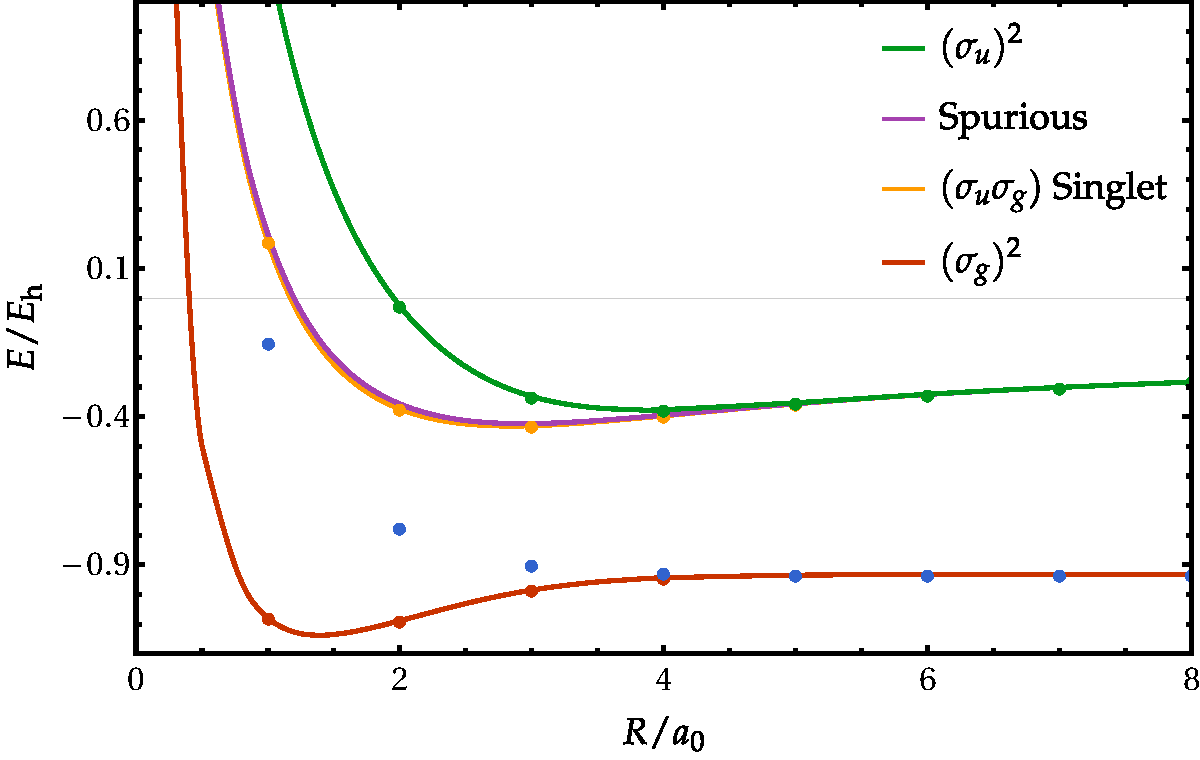
\includegraphics[width=\linewidth]{Figures/fig_1.pdf}
  \caption{
    OO-CID energies of \ce{H_2} in the STO-3G basis set with respect to the bond length $R$. The dots represent the corresponding FCI energies.
    \label{fig:fig_1}}
\end{figure}
%%% %%% %%% %%%

In this first subsection, the description of excited states outside of the CAS (or outside of the determinant expansion in the MCSCF case) is investigated.
As even the smallest non-trivial CASSCF calculation is already quite messy, we start with a minimal MCSCF example to exemplify the flexibility of these ansatze.
It is known that for the hydrogen molecule in a minimal STO-3G basis set, \cite{Hehre_1969} the two configuration interaction doubles (CID) energies correspond to the exact ground state and doubly-excited state within this basis.
The potential energy surfaces of these two states are plotted in Fig.~\ref{fig:fig_1}  (orange and green line respectively), the dots represent the corresponding FCI energies of this system.
The molecular orbitals of these two states are determined by the symmetry of the system, yet, one can still rotate them and explore the orbital-optimized (oo) CID energy landscape in search of other stationary points.
In fact, we observe that there exists an oo-CID solution (see yellow curve in Fig.~\ref{fig:fig_1}), with the energy of the exact open-shell singlet which is usually unattainable by the CID ans\"atz.
This solution is associated with spatially symmetry-broken orbitals.
Unfortunately, there is also an additional spurious non-physical oo-CID solution (purple curve) which has also symmetry-broken orbitals.
The orbitals of the four solutions are given in the \SupInf.
This simple example shows that MCSCF ansatze are flexible enough to exhibit stationary points associated with physical states outside of their ``determinant space''.
In particular, in the following we will focus on the description of excited states outside of the CAS by CASSCF wave functions.

\begin{table}
  \caption{Energies of \ce{H2} at $R=1~a_0$ using the 6-31G basis set for various formalism: FCI, SA-CASSCF with a (2,2) CAS, SA-CASSCF with a (3,2) CAS and SS-CASSCF with a (2,2) CAS.}
  \label{tab:tab_1}
  \begin{ruledtabular}
    \begin{tabular}{cccccc}
      spin & state & FCI  & SA(2,2) & SA(3,2) & SS(2,2) \\
      \hline
      \ce{Singlet}
           & 1 & -1.09897 & -1.07170 & -1.08924 & -1.09225 \\
           & Spurious &  &  &  & -1.08569 \\
           & Spurious &  &  &  & -1.07871 \\
           & 2 & -0.46395 & -0.43494 & -0.44196 & -0.46368 \\
           & 3 & -0.07450 &  & -0.06164 & -0.0594551 \\
           & 4 & 0.32015 & 0.33066 & 0.32624 & 0.31914 \\
           & Spurious &  &  &  & 0.31821 \\
           & Spurious &  &  &  & 0.31844 \\
           & Spurious &  &  &  & 0.32440 \\
           & 5 & 0.57224 &  & 0.61682 & 0.61429 \\
           & 6 & 0.86353 &  & 0.86876 & 0.86392 \\
           & Spurious &  &  &  & 0.85673 \\
           & Spurious &  &  &  & 0.86266 \\
           & Spurious &  &  &  & 0.86266 \\
           & 7 & 0.96373 &  &  & 0.91147 \\
           & 8 & 1.46479 &  &  & 1.45704 \\
           & 9 & 1.81277 &  &  & 1.80747 \\
           & 10 & 2.71948 &  &  & 2.71766 \\
           & Spurious &  &  &  & 2.70046 \\
           & Spurious &  &  &  & 2.69883 \\
      \hline
      \ce{Triplet}    
           & 1 & -0.57616 & -0.57166 & -0.57406 & -0.57417 \\
           & 2 & -0.28180 &  & -0.27990 & -0.27990 \\
           & 3 & 0.51519 &  & 0.51654 & 0.51638 \\
           & 4 & 0.62520 &  &  & 0.62401 \\
           & 5 & 1.30761 &  &  & 1.30572 \\
           & 6 & 1.61884 &  &  & 1.61685 \\
    \end{tabular}
  \end{ruledtabular}
\end{table}

Then, we stick with the hydrogen molecule but we turn to a slightly larger basis set, namely the 6-31G one, \cite{Ditchfield_1971} and consider a (2,2) CASSCF wave function.
This system can be considered as the smallest non-trivial system to investigate the CASSCF landscape.
Using SA-CASSCF one can obtain three singlet and one triplet state as shown in Table~\ref{tab:tab_1}.
On the other hand, using the same active space but in a SS formalism an approximation for each of the sixteen FCI states of this system is obtained.
Table~\ref{tab:tab_1} shows that the agreement between the SS-CASSCF energies and their FCI counterparts is consistent for all states and is still quantitative outside of the CAS.
The mean absolute deviation is $0.00250~E_h$ for the four states within the CAS and $0.01106~E_h$ for the twelve remaining states.
In addition, as expected the SS (2,2) energies are in closer agreement than the SA (2,2) ones (which have a mean absolute deviation of $0.01782~E_h$), because the orbitals are fully optimized for each states.
Even with the only non-exact larger active space available, namely (3,2), the SA formalism cannot obtain as much states as the SS one with only two active orbitals.

%%%  FIG 2  %%%
\begin{figure}
  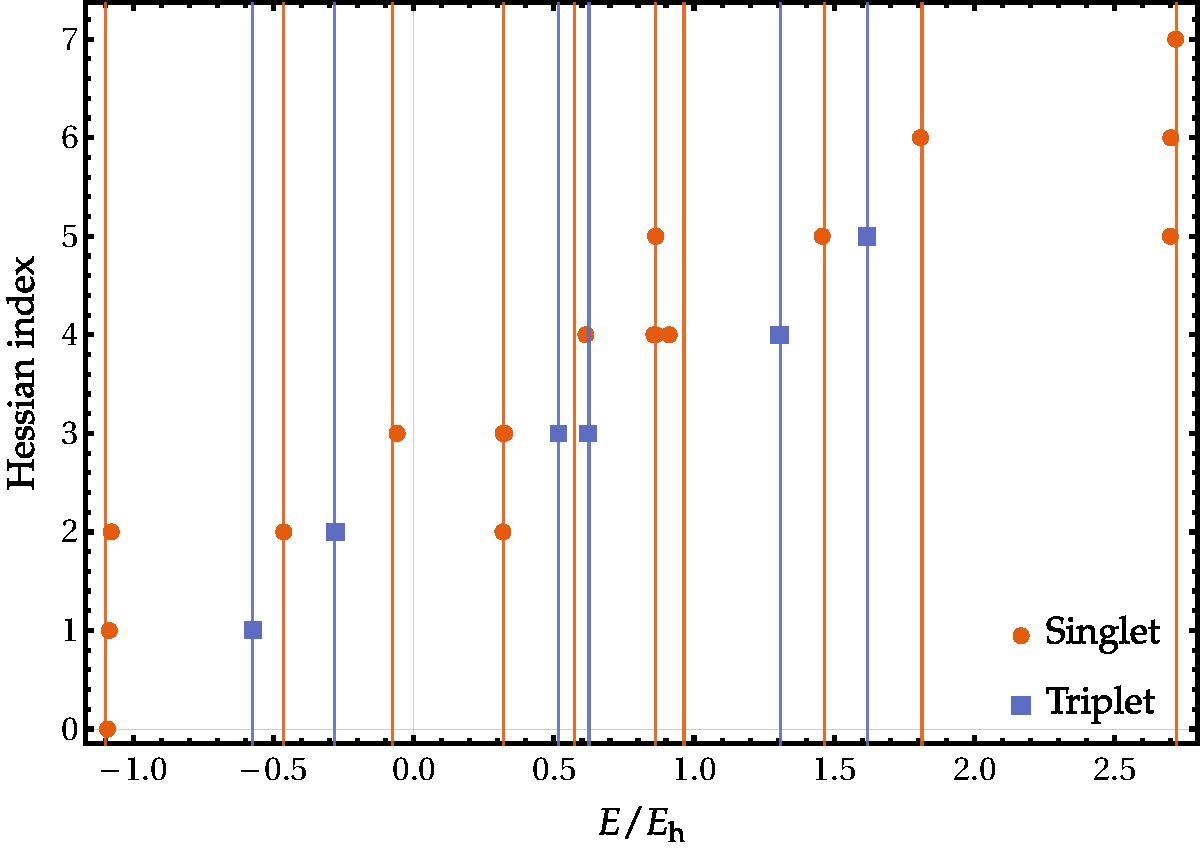
\includegraphics[width=0.9\linewidth]{Figures/fig_3a.pdf}
  \caption{Index of the SS-CASSCF solutions of \ce{H2} in the 6-31G basis set at $R=1~a_0$ with respect to their energies
    \label{fig:fig_2}}
\end{figure}
%%% %%% %%% %%%

From a landscape perspective, the simplest characterization of SS-CASSCF solutions that can be used is the Hessian index of the corresponding stationary points, \ie the number of negative eigenvalues of the Hessian.
It has also been argued that an approximation to the $n$-th excited state should be a $n$-index stationary point. \todo{ref}
Figure~\ref{fig:fig_2} shows the index of the solutions of Tab.~\ref{tab:tab_1} with respect to their energy.
First, we observe that SS-CASSCF excited states exist as saddle points on the landscape similarly to what has been observed in various other formalism. \cite{Gilbert_2008,Hait_2021,Kossoski_2021}
Then, this figure suggests that the index criteria might not be a really useful criteria for high-lying excited states.
Indeed, for example the solution with energy $2.71766~E_h$ is a good approximation to the 15th excited state while only being an index-7 stationary point.
Also, we point out that only the stationary points corresponding to excited states within the CAS are upper bound of their exact counterparts. \cite{Helgaker_2000,Mahler_2021}

%%%%%%%%%%%%%%%%%%%%%%%%%%%%%%%%%%%%%%%%%%%%%%%%%%
\subsection{SS-CASSCF spurious solutions}
\label{sec:spurious}
%%%%%%%%%%%%%%%%%%%%%%%%%%%%%%%%%%%%%%%%%%%%%%%%%%

Because there is no free lunch, there is a counterpart to these advantages of SS-CASSCF.
Indeed, in this case four singlet states exhibit close-lying spurious solutions (see Table~\ref{tab:tab_1}).
These four singlet states correspond to the singlet closed-shells of the system.
We should also mention that there may be other spurious solutions that have been missed by our grid-based search.
Figure~\ref{fig:fig_2} demonstrates that close-lying spurious solutions may have different indexes.
For example, the three lowest solutions have indexes equal to 0, 1 and 2 in ascending order of energy.
At this stage, one can argue that in terms of energy spurious solutions are not that much worrying as each of them is fairly close to an FCI energy (vertical lines in  Fig.~\ref{fig:fig_2}).

%%%  FIG 3  %%%
\begin{figure}
  \begin{subfigure}[l]{0.45\linewidth}
    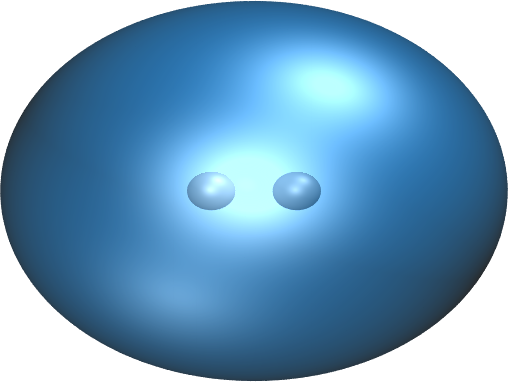
\includegraphics[width=0.75\linewidth]{Figures/h2_HF_mo1.cube.png}
    \caption*{\centering $(1\sigma_g)~n_\text{occ}~=~1.9998$}
  \end{subfigure}
  \begin{subfigure}[r]{0.45\linewidth}
    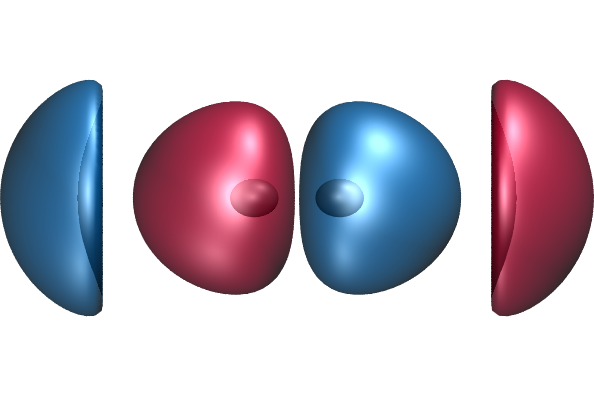
\includegraphics[width=0.75\linewidth]{Figures/h2_HF_mo4.cube.png}
    \caption*{\centering $(2\sigma_g)~n_\text{occ}~=~0.0002$}
  \end{subfigure}
  $E=-1.07871~E_h$
  
  \begin{subfigure}[l]{0.45\linewidth}
    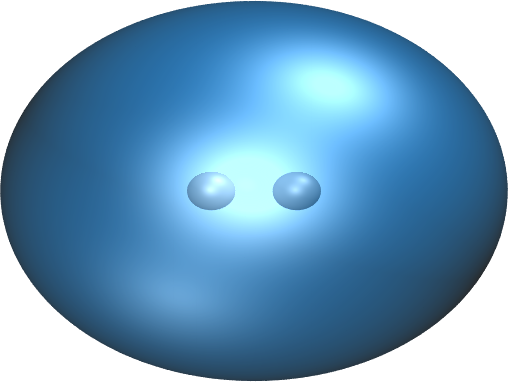
\includegraphics[width=0.75\linewidth]{Figures/h2_HF_mo1.cube.png}
    \caption*{\centering $(1\sigma_g)~n_\text{occ}~=~1.993$}
  \end{subfigure}
  \begin{subfigure}[r]{0.45\linewidth}
    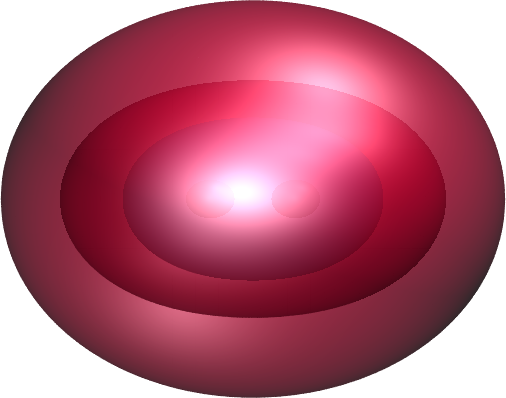
\includegraphics[width=0.75\linewidth]{Figures/h2_HF_mo3.cube.png}
    \caption*{\centering $(2\sigma_g)~n_\text{occ}~=~0.007$}
  \end{subfigure}
  $E=-1.08569~E_h$
  
  \begin{subfigure}[l]{0.45\linewidth}
    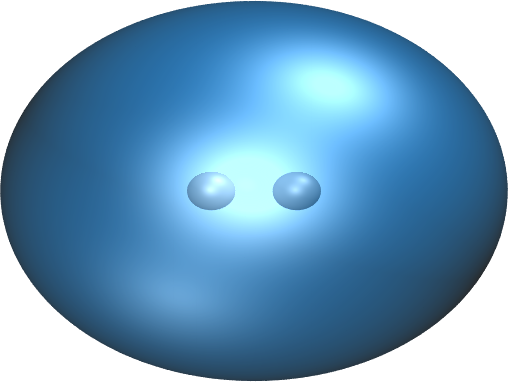
\includegraphics[width=0.75\linewidth]{Figures/h2_HF_mo1.cube.png}
    \caption*{\centering $(1\sigma_g)~n_\text{occ}~=~1.989$}
  \end{subfigure}
  \begin{subfigure}[r]{0.5\linewidth}
    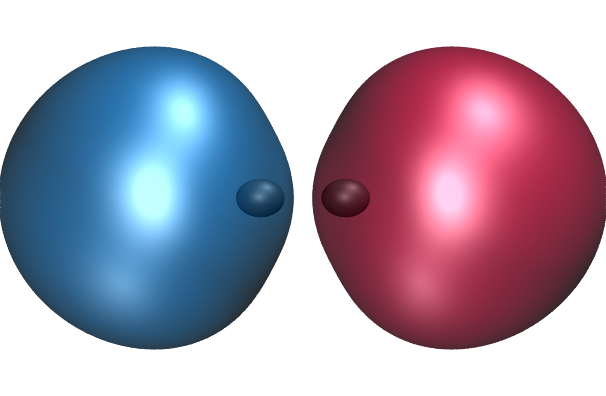
\includegraphics[width=0.75\linewidth]{Figures/h2_HF_mo2.cube.png}
    \caption*{\centering $(2\sigma_g)~n_\text{occ}~=~0.011$}
  \end{subfigure}
  $E=-1.09225~E_h$
  
  \caption{Natural orbitals of the three lowest (2,2) SS-CASSCF singlet solutions of \ce{H2} at $R=1~a_0$ \label{fig:fig_3}}
\end{figure}
%%% %%% %%% %%%

A practical and robust SS-CASSCF should avoid these spurious solutions, thus understanding their cause of appearance would facilitate design of SS algorithms.
Therefore examining the difference between close-lying solutions should shed light on the physical phenomena causing their appearance.
We start by focusing on the two spurious solutions lying close to the ground state for the hydrogen molecule in the 6-31G basis set (see Table~\ref{tab:tab_1}).
Figure~\ref{fig:fig_3} shows the natural orbitals (in the active space) and their occupancies for these three solutions.
Note that because there are only two orbitals in the active space, only two orbitals can have a non-zero occupation.
We know that at $R=1~a_0$ the HF ground state, corresponding to a single determinant with two electrons in the $(1g)$ orbital, is a reasonable approximation of the FCI ground state.
We can see that these three solutions have almost two electrons in the $(1g)$ orbital which is in agreement with the performance of HF.
The difference between these solutions is the orbital in which the remaining small fractional occupation is put.
The three solutions correspond to the three possible choices of virtual orbital to be put in the active space.
We observe the same phenomenon for the three other closed-shell states.
In each case, we have a dominant single configuration dynamically correlated by a small occupation in one of the three other remaining orbitals.
For the two intermediate closed-shell states the fourth closely-lying solution correspond to a spatially symmetry-broken solution.
In both cases, the symmetry-broken solution is the closest to the FCI energy among the four solutions.

\begin{table}[b]
  \caption{Ground-state (2,2) SS-CASSCF energies of \ce{H2} at $R=1~a_0$ using the 6-311G basis set and its FCI counterpart.}
  \begin{ruledtabular}
    \label{tab:tab_2}
    \begin{tabular}{llllll}
      SS(1,2)~(HF) & -1.08025 & & & &\\
      \hline
      SS(2,2) & -1.09429 & -1.08866 & -1.08074 & -1.08033 & -1.08026 \\
      \hline
      SS(3,2) & -1.095 & -1.09436 & -1.09429 & -1.08904 & -1.08886 \\
                   & -1.08867 & -1.08082 & -1.08075 & -1.08034 & \\
      \hline
      SS(4,2) & -1.10251 & -1.10196 & -1.09507 & -1.095 & -1.09437 \\
          & -1.08923 & -1.08905 & -1.08886 & -1.08083 &  \\
      \hline
      SS(5,2) & -1.10267 & -1.10251 & -1.10213 & -1.09507 & -1.08924 \\
      \hline
      SS(6,2)~(FCI) & -1.10267 & & & &\\
    \end{tabular}
  \end{ruledtabular}
\end{table}

Therefore, these first results seem to suggest that multiple CASSCF solutions arise from a freedom in the choice of virtual orbitals which will bring dynamical correlation.
The remainder of this subsection is concerned with confirming this result.
We consider again the \ce{H2} molecule at $R=1~a_0$ with a (2,2) CAS but in the slightly larger 6-311g basis set (three basis function per hydrogen atom). \cite{Krishnan_1980}
In this case five close-lying solutions has been found for the ground state, the energies of these states are given in Table~\ref{tab:tab_2}.
From what has been seen before (see Fig.~\ref{fig:fig_3}), this could have been expected as there are five possible virtual orbitals that can be chosen as the active orbital that dynamically correlates the HF ground-state determinant.
For higher energies, the spectrum exhibit five other groups of five or six close-lying solutions, which correspond once again to the five closed-shell excited states.
The sixth state, when present, corresponds to a spatially symmetry-broken solution as observed in the smaller 6-31g basis set (see Tab.~\ref{tab:tab_1}).
Therefore, because spurious solutions correspond to different possible choices for orbitals in the active space, the number of such solutions should be expected to grow combinatorially with respect to the size of the basis set.

To further illustrate this result, we consider the case of larger active spaces.
Table~\ref{tab:tab_2} also shows the number of ground-state solutions in the 6-311g basis set for increasing active spaces.
We know that in the limiting case of the largest possible active space, which is equivalent to FCI, there is only one ground-state solution.
If the active space contains five orbitals, we find five solutions which is consistent with choosing four out of five virtual orbitals to put in the active space.
The binomial coefficient corresponding to choosing two (or three) orbitals out of five gives ten possibilities.
However, we have found only nine solutions in both cases.
There might be a tenth solution that have been missed by our grid-based search.
Fig.~\ref{fig:fig_3} shows that the fractional occupation is becoming really small when the highest virtual orbital is chosen.
Therefore, choices of orbitals with very small contribution might be harder to converge toward and hence less preoccupying in practice.

\begin{table}
  \caption{Four lowest singlet FCI states of \ce{H2} at $R=1~a_0$ using the 6-31G basis set and their (3,2) SS-CASSCF counterpart. States 1 and 4 are closed-shell while 2 and 3 correspond to open-shells.}
  \begin{ruledtabular}
    \label{tab:tab_3}
    \begin{tabular}{cllll}
      state & 1  & 2 & 3 & 4 \\
      \hline
      FCI & -1.09897 & -0.46395 & -0.07450 & 0.32015 \\
      \hline
      SS(2,2) & -1.09225 & -0.46368 & -0.0594551 & 0.31914 \\
            & -1.08569 &  &  & 0.31821 \\
            & -1.07871 &  &  & 0.31844 \\
            &  &  &  & 0.32440 \\
      \hline
      SS(3,2) & -1.09875 & -0.463822 & -0.0711398 & 0.315896 \\
            & -1.09256 & -0.463689 & -0.0632185 & 0.320249 \\
            & -1.08581 &  & -0.0594551 & 0.322577 \\
    \end{tabular}
  \end{ruledtabular}
\end{table}

We turn to the influence of increasing the active space on excited states.
To exemplify this, Tab.~\ref{tab:tab_3} shows the (3,2) SS-CASSCF solutions for the four lowest FCI states of \ce{H2} at $R=1~a_0$ using the 6-31G basis set.
Once again, the three ground-state solutions correspond to the three possible choices of two virtual orbitals out of three to fill out the active space.
For the first excited closed-shell state we have found the three solutions analog to the ones of the ground state.
No symmetry-broken solution has been obtained for this state as opposed to the case of the (2,2) active space (see Table~\ref{tab:tab_1}).
Our grid-based approach may have missed this solution or this larger active space might give enough flexibility so that breaking the symmetry is not needed.

Now turning to the open-shell singlets, which do not exhibit close-lying spurious solutions when one use two active orbitals.
An open-shell state need for a proper minimal description at least two orbitals, one for each electron.
Therefore if the active space contains only two orbitals there is no freedom in the choice of orbitals once the two singly-occupied active orbitals have been chosen.
On the other hand, adding an orbital to the active space gives freedom in the choice of the virtual orbital to add to the active space to dynamically correlate the open-shell, resulting in spurious close-lying open-shell solutions.
Table~\ref{tab:tab_3} shows that indeed the open-shell states also exhibit close-lying spurious solutions when the active space is enlarged.

%%% FIG 4  %%%
\begin{figure}
  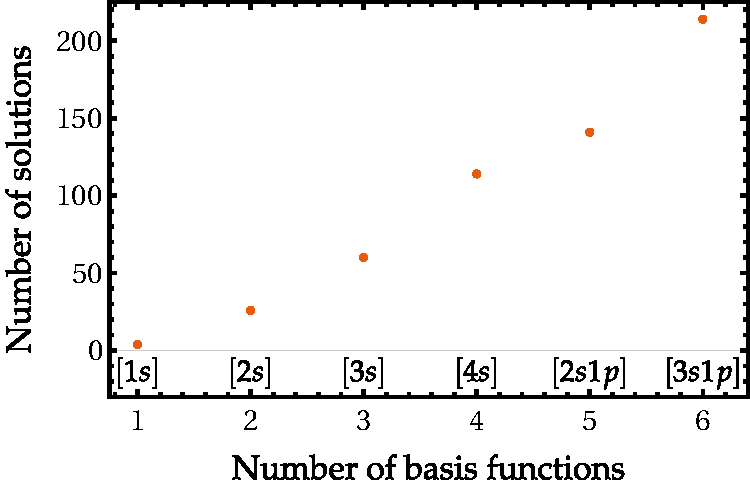
\includegraphics[width=0.9\linewidth]{Figures/fig_2a.pdf}
  \caption{Number of (2,2) SS-CASSCF solution with respect to the size of the basis set for \ce{H2} at $R=1~a_0$. \label{fig:fig_4}}
\end{figure}
%%% %%% %%% %%%

Finally, we have seen that the number of solutions is expected to grow combinatorially.
To exemplify that the number of SS-CASSCF solutions should be expected to be really large in real system, we show the number of solutions with respect to increasing size of basis set.
Figure~\ref{fig:fig_4} shows it in the case of a (2,2) CASSCF ans\"atz for the hydrogen molecule at $R=1~a_0$.
As expected, the number of solutions is growing incredibly fast.
In addition, note that the growth is not smooth when basis functions with different symmetries are added.
This might be due to the fact some choices of virtual orbitals for the active space are not possible due to symmetry.

%%%%%%%%%%%%%%%%%%%%%%%%%%%%%%%%%%%%%%%%%%%%%%%%%%
\subsection{SS-CASSCF solution space and static correlation}
\label{sec:static}
%%%%%%%%%%%%%%%%%%%%%%%%%%%%%%%%%%%%%%%%%%%%%%%%%%

%%% FIG 5  %%%
\begin{figure}
  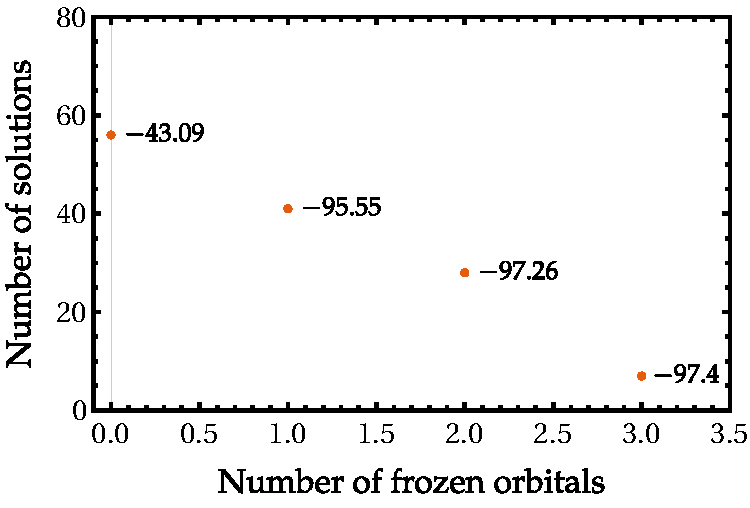
\includegraphics[width=0.9\linewidth]{Figures/fig_2b.pdf}
  \caption{Number of (2,2) SS-CASSCF solution with respect to the \ce{H2} bond length $R$ in the 6-31G basis set. \label{fig:fig_5}}
\end{figure}
%%% %%% %%% %%%

It is now well-known that the number of solution in HF, DFT and CC is not constant with respect to variation of the geometry of the system. \todo{ref}
In this section, the influence of geometry, and therefore of static correlation, on the SS-CASSCF solution space and its landscape will be investigated.
Figure~\ref{fig:fig_5} shows the number of solution (2,2) SS-CASSCF solutions for \ce{H2} in the 6-31G basis set with respect to the bond length $R$.
One can immediately see that the same behavior as in the aforementioned theories is observed in the context of CASSCF, namely that the number of solutions is larger when the static correlation becomes dominant.
Indeed, the number of solution is growing when the correlation is getting stronger, \ie when we stretch the bond.
Therefore, the focus of this section will be to understand the origin and the behavior of these additional, spurious or not, solutions.

%%%  FIG 6  %%%
\begin{figure}
  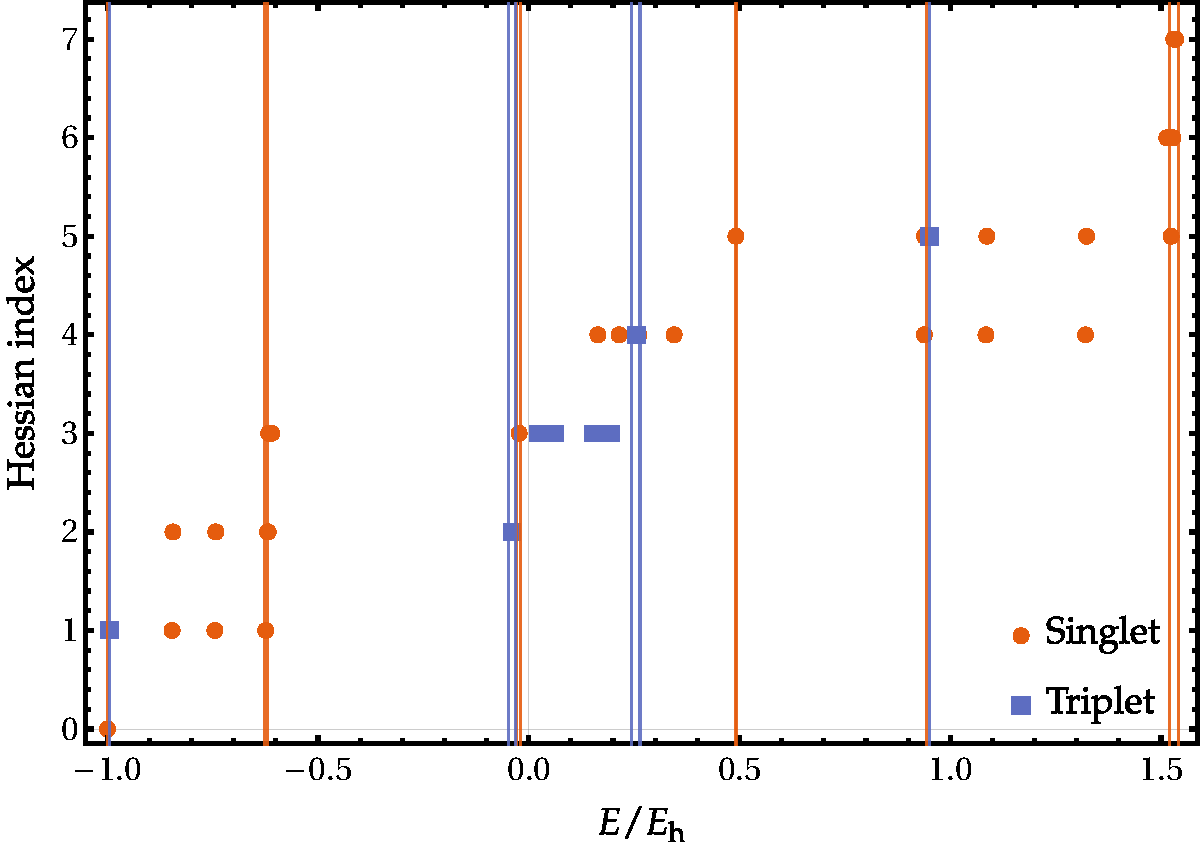
\includegraphics[width=0.9\linewidth]{Figures/fig_3b.pdf}
  \caption{Index of the SS-CASSCF solutions of \ce{H2} in the 6-31G basis set at $R=5~a_0$ with respect to their energies
    \label{fig:fig_6}}
\end{figure}
%%% %%% %%% %%%

Once again, we start by looking at the index of the stationary points, Fig.~\ref{fig:fig_6} is the analog of Fig.~\ref{fig:fig_2} but in the strong correlation regime ($R=5~a_0$).
The first thing to notice is that now some spurious solutions are not close to any FCI energy.
Therefore one can argue that these solutions are much more preocuppying than in the dynamic correlation regime where spurious solutions are still fairly good approximations of exact states.
However, all FCI energies remain approximately matched by at least one CASSCF solution.
So the problem of spurious solutions seems more serious in the strong correlation regime, which could have been expected as it has already been observed in the HF and CC contexts. \todo{ref}

%%%  FIG 7  %%%
\begin{figure}
  \centering
  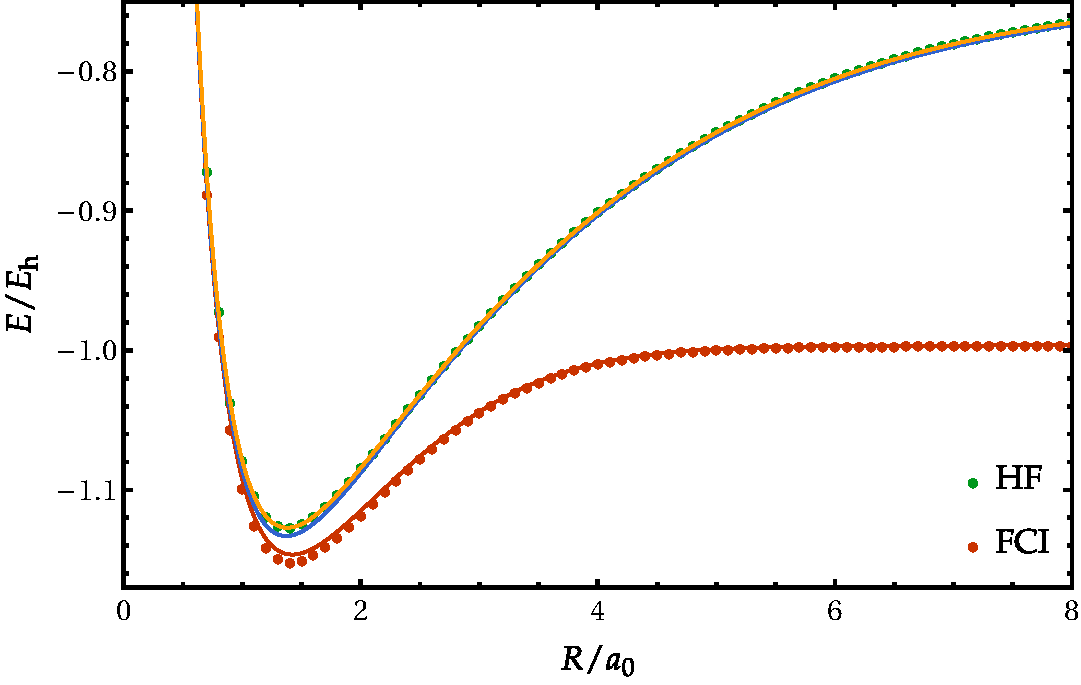
\includegraphics[width=0.9\linewidth]{Figures/fig_5.pdf}
  \caption{Potential energy curves of the three lowest (2,2) SS-CASSCF singlet states (lines) for \ce{H2} in the 6-31G basis set (see Tab.~\ref{tab:tab_1}). The dots correspond to the FCI and HF ground states. \label{fig:fig_7}}
\end{figure}
%%% %%% %%% %%%

These preoccupying spurious solutions can be understood by looking at the evolution of the multiple solutions at equilibrium/
Figure.~\ref{fig:fig_7} depicts the potential energy curves associated with the three lowest solutions at equilibrium (see Fig.~\ref{fig:fig_3} for canonical orbitals at equilibrium).
One can immediately see that only one of these solutions goes to the correct ground-state FCI dissociation limit.
This solution is the lowest one at $R=1~a_0$ and has a fractional occupation in the $(1\sigma_u)$ orbital.
At dissociation, the configuration of this solution is $1(\sigma_g)1(1\sigma_u)$.
On the other hand, the two other solutions configuration are $1.997(1\sigma_g)0.003(2\sigma_g)$ and $1.999(1\sigma_g)0.001(2\sigma_u)$, respectively.
This is due to the fact that the additional active orbital does not have the required symmetry to mix with the $(1g)$ orbital to produce the correct dissociation limit.
As a consequence these solutions only have an energy slightly below the HF dissociation limit as they recover only a small amount of dynamical correlation energy.
So we can already say that some spurious solutions completely off from FCI energies in Fig.~\ref{fig:fig_6} correspond to wrong HF dissociation limits.
It is interesting to note that these solutions preserve the character of the active orbitals along the PES.
Indeed, one could have thought that the orbital with the wrong symmetry could have been swapped with the $(1\sigma_u)$ orbital to achieve the correct dissociation limit.
Therefore, it seems that the SS-CASSCF solutions possess some kind of diabaticity.
Section~\ref{sec:avoided} will further illustrate this.

%%%  FIG 8  %%%
\begin{figure}
  \centering
  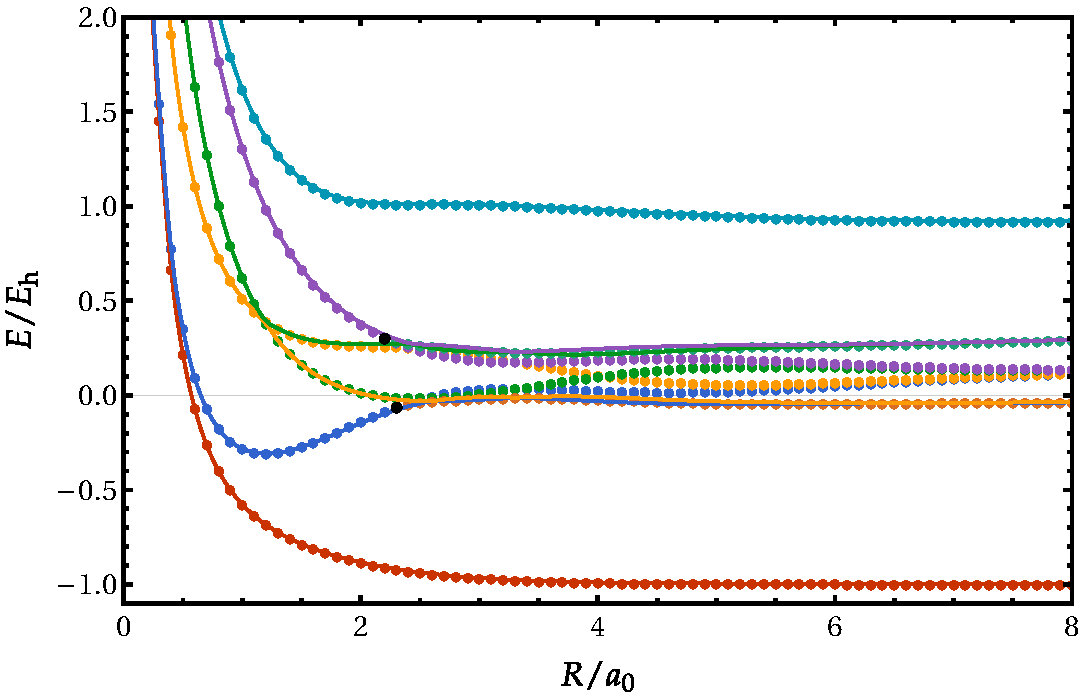
\includegraphics[width=0.9\linewidth]{Figures/fig_6.pdf}
  \caption{Potential energy curves of the (2,2) SS-CASSCF triplet states of \ce{H2} in the 6-31G basis set. \label{fig:fig_8}}
\end{figure}
%%% %%% %%% %%%

At this point we still need to understand the origin of the additional solutions appearing in the strong correlation limit.
To investigate this we plot the potential energy curves of the (2,2) SS-CASSCF triplet states of the system in Figure~\ref{fig:fig_8}.
Table~\ref{tab:tab_1} has shown that at equilibrium there are six CASSCF triplet solutions which are all quantitative approximations of one of the six FCI triplets.
However, one can see in Fig.~\ref{fig:fig_8} that the four intermediate solutions are going to the same unphysical dissociation limit (see the four FCI dissociation limits represented by the dots).
On the other hand, the lowest and highest CASSCF triplets are in agreement with their FCI counterpart at all bond lengths.
At $R\simeq 2.3~a_0$ and $R\simeq 2.4~a_0$ (black dots), two additional CASSCF triplet solutions appear and these solutions go to the two distinct correct dissociation limits (orange and light green dots).
These two solutions are spin pure ($\expval{S^2}=2$) but their natural orbitals are spatially symmetry-broken (see \SupInf).
So these black dots correspond to CASSCF Coulson-Fisher points analogous to the infamous one in the context of HF.

The situation for the six open-shell singlets is completely analog, \ie the four intermediate solutions at $R=1~a_0$ evolve to an unphysical dissociation limit and two spatially symmetry-broken open-shell singlets appear.
The corresponding potential energy surfaces and natural orbitals are given in the \SupInf.
Therefore, one source of additional solutions in the strong correlation regime is symmetry breaking which is completely analog to what is observed in HF. \todo{ref}
Yet, because the CASSCF ans\"atz is much more flexible than one single determinant, CASSCF symmetry breaking should be expected to be less common than in HF.
Moreover, enlarging the active space, hence increasing the flexibility of the ans\"atz, should allow the description of the difficult states without resorting to symmetry-breaking.

Finally, the behavior of the three closed-shell excited-state solutions is discussed.
For the symmetry-adapted solutions (three per closed-shell, see discussion of Fig.~\ref{fig:fig_3}), this is completely analogous to the case of the ground state discussed in details above (see Fig.~\ref{fig:fig_5}), \ie only one solution out of the three close-lying ones is going to the corresponding FCI dissociation limit.
The two spatially symmetry-broken closed-shell found at $R=1~a_0$ also evolve to their respective correct dissociation limit.
For the second closed-shell excited state (state 6 in Table~\ref{tab:tab_1}), we have found a degenerate spin symmetry-broken solution.
In fact, the associated exact solution is degenerate with a triplet at dissociation limit.
So the spin symmetry-broken solution correspond to a combination of these degenerate singlet and triplet.
Degeneracy of a singlet and a triplet state at dissociation resulting in the possibility of converging toward a spin symmetry-broken mix is also a cause of additional SS-CASSCF solutions.

Finally, several spatially symmetry-broken solutions with a dominant single-determinant configuration has been found close to the first and third closed-shell excited-state dissociation limits (states 4 and 10).
This is consistent with the fact that HF can describe these two dissociation limits with one spatially symmetry-broken single determinant. \todo{Do we have a ref for this? First year PhD report?}
On the other hand, the CASSCF ans\"atz can represent these two states in an alternative way without resorting to symmetry-breaking.
Indeed, by putting the two electrons in two different orbitals, SS-CASSCF can represent these two anti-bonding closed-shells (see \SupInf~for the corresponding natural orbitals).
These two ways of representing the same state gives the last cause of appearance of additional solutions in the strong correlation regime in this system.

%%%%%%%%%%%%%%%%%%%%%%%%%%%%%%%%%%%%%%%%%%%%%%%%%%
\subsection{Avoided crossing}
\label{sec:avoided}
%%%%%%%%%%%%%%%%%%%%%%%%%%%%%%%%%%%%%%%%%%%%%%%%%%

%%%  FIG 9  %%%
\begin{figure}
  \centering
  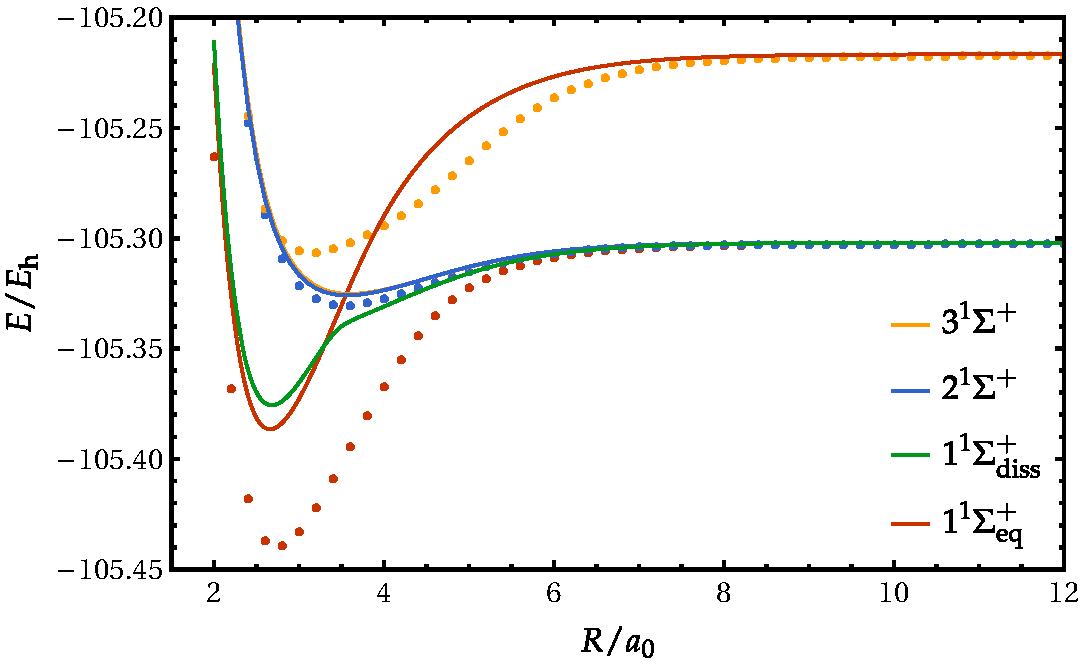
\includegraphics[width=0.9\linewidth]{Figures/fig_7.pdf}
  \caption{Potential energy curves of the SS-CASSCF states of \ce{LiF} in the STO-3G basis set. \label{fig:fig_9}}
\end{figure}
%%% %%% %%% %%%

In this last section the description of avoided crossings at the SS-CASSCF level will be investigated.
It has been shown that HF solutions behave ``quasi-diabatically'' in the vicinity of avoided crossings, \ie they cross instead of avoiding each other. \cite{Thom_2009}
One can recover the avoided crossing by making interact the HF solutions through the Hamiltonian, resulting in a non-orthogonal (NO) CI scheme. \cite{Burton_2019}
Therefore, it would be interesting to see if SS-CASSCF solutions also behave ``quasi-diabatically'' or if they can reproduce the avoided crossing.
To answer this question we investigate the LiF molecule in the STO-3G basis set.
The ionic ground state of this molecule at equilibrium undergoes an avoided crossing with a covalent excited state when the bond is stretched. \cite{Thom_2009,Mahler_2021}

First, the focus is on the sole ground-state which is a closed-shell ionic state at equilibrium and which dissociates into two neutral open-shell atoms.
The single determinant HF ground-state gives a fairly good description of the equilibrium closed-shell.
However, this HF solution cannot describe the correct dissociation limit which is inherently multi-reference. \todo{add ref}
Figure~\ref{fig:fig_9} shows the lowest (2,2) SS-CASSCF singlet solutions (lines) as well as the three lowest FCI singlets (dots).
The SS-CASSCF ground-state solution at equilibrium (red curve) correspond to a dynamically correlated HF ground state, \ie the active space contains the HF highest occupied MO, a $\pi_y$ orbital mostly localized on the fluorine atom, and the associated $\pi_y^*$.
By delocalizing a small fraction of electron in the $\pi_y^*$ orbital the SS-CASSCF solution achieve some resonance stabilization between the HF ground state and the singlet charge-transfer excited state.
However, this solution is going to the wrong dissociation limit as we can see on the plot.

We have found another minimum solution at dissociation limit (green curve).
This solution correspond to the two open-shell atom, the active space has one electron in the $2s$ of the lithium atom and one electron in the $\pi_z$ localized on the fluorine.
When $R$ decrease the electron in the $2s$ is transfered to the $\pi_z$ and at equilibrium this solution is equivalent to the closed-shell HF ground state.
The $2s$ orbital localized on the Lithium atom does have the correct symmetry to dynamically correlate the HF determinant as the $1 {}^1\Sigma^+_{\text{eq}}$.

Now turning to the SS-CASSCF description of the avoided crossing.
Figure~\ref{fig:fig_9} shows that the CASSCF singlet states are behaving in a ``quasi-diabatic'' manner.
The two singlet excited states (yellow and purple curves) are dissociating to the lowest dissociation limit whereas one of them should interact with the ground-state to form an avoided crossing.
It would be interesting to make interact these three solutions through the Hamiltonian in a NOCI scheme for multi-reference solutions.
By scrutinizing the symmetry of the natural orbitals of the two singlet excited states, we expect that only one of them can interact with the ground state (see \SupInf).
It would also be interesting to see if one can describe the ground state at all bond lengths by interaction of the $1 {}^1\Sigma^+_{\text{eq}}$ and $1 {}^1\Sigma^+_{\text{diss}}$ solutions correct at small and large $R$, respectively.
We keep this for a future work.
An alternative way to describe this avoided crossing at the CASSCF level would be to increase the active space.
Indeed,iIf the CASSCF states possess some form of diabaticity which prevent them from swapping active and virtual orbitals along the potential energy curves, including all the necessary orbitals to describe the binding curve would fix this problem. 

%%%%%%%%%%%%%%%%%%%%%%%%%%%%%%%%%%%%%%%%%%%%%%%%%%
\subsection{(Core excitations)}
\label{sec:core}
%%%%%%%%%%%%%%%%%%%%%%%%%%%%%%%%%%%%%%%%%%%%%%%%%%

%%% FIG 2  %%%
\begin{figure}
  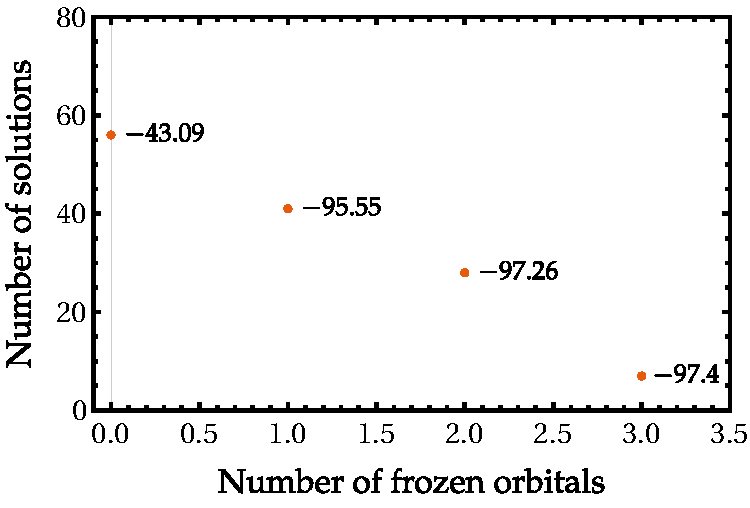
\includegraphics[width=0.9\linewidth]{Figures/fig_2c.pdf}
  \caption{Number of SS-CASSCF solution with respect to various parameters of the system. Left: Influence of the size of the basis set for \ce{H2} at $R=1~a_0$. Middle: Influence of the geometry for \ce{H2} in 6-31G basis set. Right: Influence of freezing core orbitals for the \ce{HF} molecule at $R=2~a_0$ in STO-3G basis set. \label{fig:fig_9}}
\end{figure}
%%% %%% %%% %%%

Finally, we look at the influence of frozen core orbitals on the number of CASSCF solution.
The right plot of Fig.~\ref{fig:fig_2} shows the number of solution for the HF molecule at $R=2~a_0$ in the STO-3G basis set.
We see that the number of solution is decreasing each time we freeze one more orbital.
In addition, the energy of the highest solution (value in Hartree next to each dot) is also lower when core orbitals are frozen.
These two results were expected as the same trends were observed in the context of Hartree-Fock theory. \cite{Dong_2020}
We believe that one could take advantage of this property to target effectively core excited states at the SS-CASSCF level.


%=================================================================%
\section{Conclusion}
\label{sec:conclusion}
%=================================================================%

\todo{Add conclusion}

Talk about how to choose the physical solution, spin symmetry breaking, neuscamman's multiple solution.


%%%%%%%%%%%%%%%%%%%%%%%%
\begin{acknowledgements}
%%%%%%%%%%%%%%%%%%%%%%%%
\todo{Add acknowledgements}
%%%%%%%%%%%%%%%%%%%%%%
\end{acknowledgements}
%%%%%%%%%%%%%%%%%%%%%%

\appendix

%%%%%%%%%%%%%%%%%%%%%%%%%%%%%%%%%%%%%%
\section{Gradient and Hessian matrix elements}
\label{app:appendixA}
%%%%%%%%%%%%%%%%%%%%%%%%%%%%%%%%%%%%%%

In this appendix we give explicit expressions to compute the gradient and Hessian used in the Newton-Raphson algorithm.
The gradient can be divided in two parts, namely the CI part $g^c$ and the orbital part $g^o$.
This latter can be divided further in three parts corresponding to the non-redundants rotations for a CASSCF wave function: core-active, core-virtual and active-virtual.

\begin{align}
  \label{eq:CASSCF_CI_Gradient}
  g^c_{K} &= \eval{\mleft(\pdv{E}{S_{K}}\mright)}_{\bm{\lambda}=0} = \mel**{\Psi_0}{\com{\hH}{\hS}}{\Psi_0} \\
          &= 2\mel**{\Psi_K}{\hH}{\Psi_0} \notag \\
          &= 2\sum_{IJ}C_{K,I}^*\mel{I}{\hH}{J}C_{0,J} \notag
\end{align}

\begin{equation}
  \label{eq:CASSCF_Orb_Gradient_general}
  g^o_{pq} = \eval{\mleft(\pdv{E}{\kappa_{pq}}\mright)}_{\bm{\lambda}=0} = \mel**{\Psi_0}{\com{\hH}{\hK}}{\Psi_0}
\end{equation}

\begin{subequations}
  \label{eq:CASSCF_Orb_Gradient}
  \begin{align}
    g^o_{ai} &= 4(\FC{ai} + \FA{ai}) \\
    g^o_{ti} &= 4(\FC{ti} + \FA{ti}) - 2\sum_v \gamma_{tv}\FC{iv} -4\sum_{vxy}\Gamma_{tvxy}\braket{ix}{vy} \\
    g^o_{at} &= 2\sum_v \gamma_{tv}\FC{av} + 4\sum_{vxy}\Gamma_{tvxy}\braket{ax}{vy}.
  \end{align}
\end{subequations}
where we have introduced the core and active parts of the generalized Fock matrix
\begin{align}
  \label{eq:CoreActGeneralizedFock}
  \FC{pq} &= h_{pq} + \sum_{i} 2\ceri{pq}{ii} - \ceri{pi}{iq} \\
  \FA{pq} &= \sum_{vx}\gamma_{vx}(\ceri{pq}{vx} - \frac{1}{2}\ceri{px}{vq})
\end{align}

Similarly, we can divide the Hessian in three parts: CI-CI $H^{cc}$, Orb-Orb $H^{oo}$ and Orb-CI $H^{oc}$. The CI-Orb part is equivalent to the latter up to a transposition.

\begin{align}
  \label{eq:CASSCF_CICI_Hessian}
  H^{cc}_{K,L} &= \eval{\mleft(\pdv{E}{S_{K}}{S_{L}}\mright)}_{\bm{\lambda}=0} = \mel**{\Psi_0}{\com{\com{\hH}{\hS}}{\hS}}{\Psi_0} \\
  &= 2\mel**{\Psi_K}{\hH - E_0}{\Psi_L} \notag \\
  &= 2\sum_{IJ}C_{K,I}^*\mel**{I}{\hH}{J}C_{L,J} - E_0\delta_{K,L} \notag
\end{align}

\begin{align}
  \label{eq:CASSCF_OrbCI_Hessian}
  H^{oc}_{pq,K} &= \eval{\mleft(\pdv{E}{\kappa_{pq}}{S_{K}}\mright)}_{\bm{\lambda}=0} = \mel**{\Psi_0}{\com{\com{\hH}{\hK}}{\hS}}{\Psi_0} \\
                &= \mel**{\Psi_K}{\com{\hH}{E_{pq}^-}}{\Psi_0} \notag \\
                &= 2\sum_{IJ}C_{K,I}^*\mel{I}{\com{\hH}{E_{pq}^-}}{J}C_{0,J} \notag
\end{align}
where we have introduced $E_{pq}^- = \cre{p}\ani{q} - \cre{q}\ani{p}$ the anti-symmetrized spin-averaged excitation operator.
\begin{align}
  \label{eq:MCSCF_SO_OrbOrb_Hessian}
  H^{oo}_{pq,rs} &= \eval{\mleft(\pdv{E}{\kappa_{pq}}{\kappa_{rs}}\mright)}_{\bm{\lambda}=0} = \mel**{\Psi_0}{\com{\com{\hH}{\hK}}{\hK}}{\Psi_0} \\
                   &= \frac{1}{2}(1+P_{pq,rs})\mel**{\Psi_0}{\com{\com{\hH}{E_{pq}^-}}{E_{rs}^-}}{\Psi_0} \notag
\end{align}

%%%%%%%%%%%%%%%%%%%%%%
\bibliography{MCSCF_LSP}
%%%%%%%%%%%%%%%%%%%%%%

\end{document}
